\documentclass[12 pt,a4 paper ]{scrreprt}
 
\usepackage[utf8]{inputenc}
\usepackage[naustrian]{babel}
\usepackage{lmodern}
\usepackage[T1]{fontenc}
\usepackage{graphicx}
\usepackage{amsmath}
\usepackage{float}
\usepackage{amsmath,amssymb,amstext}
\usepackage{pgfplots}

\usepackage{nicefrac}
\usepackage{units}
%\usepackage[tight]{units}
%\usepackage[loose]{units}







\usepackage[headsepline,plainheadsepline]{scrpage2}
\pagestyle{scrheadings}
\ihead[\rightmark]{\rightmark} \chead[]{}
%\ohead[\pagemark]{\pagemark} \cfoot[]{}

\automark{chapter}
\renewcommand{\chaptermark}[1]{\markright{\ #1}}


\pgfplotsset{width=10cm,compat=1.6}

% for dvipdfm:
% \def\pgfsysdriver{pgfsys-dvipdfm.def}
\usepackage{pgfplots}
%\pgfplotsset{compat=1.6}% <-- moves axis labels near ticklabels (respects tick label widths)
\begin{document}


\begin{figure}
\begin{center}


\centering
\begin{tikzpicture}
\begin{axis}[
xlabel=time,
ylabel=$a$ error]
\draw[very thin,color=gray] (-0.1,-1.1) grid (3.9,3.9);
\addplot table[x=time,y=a] {daten.dat};
\addplot table[x=time,y=b] {daten.dat};
\addplot table[x=time,y=c] {daten.dat};
\addplot table[x=time,y=d] {daten.dat};
\end{axis}
\end{tikzpicture}


\caption{listige Dinge}
\label{kanne}
\end{center}
\end{figure}




\begin{figure}
\begin{center}
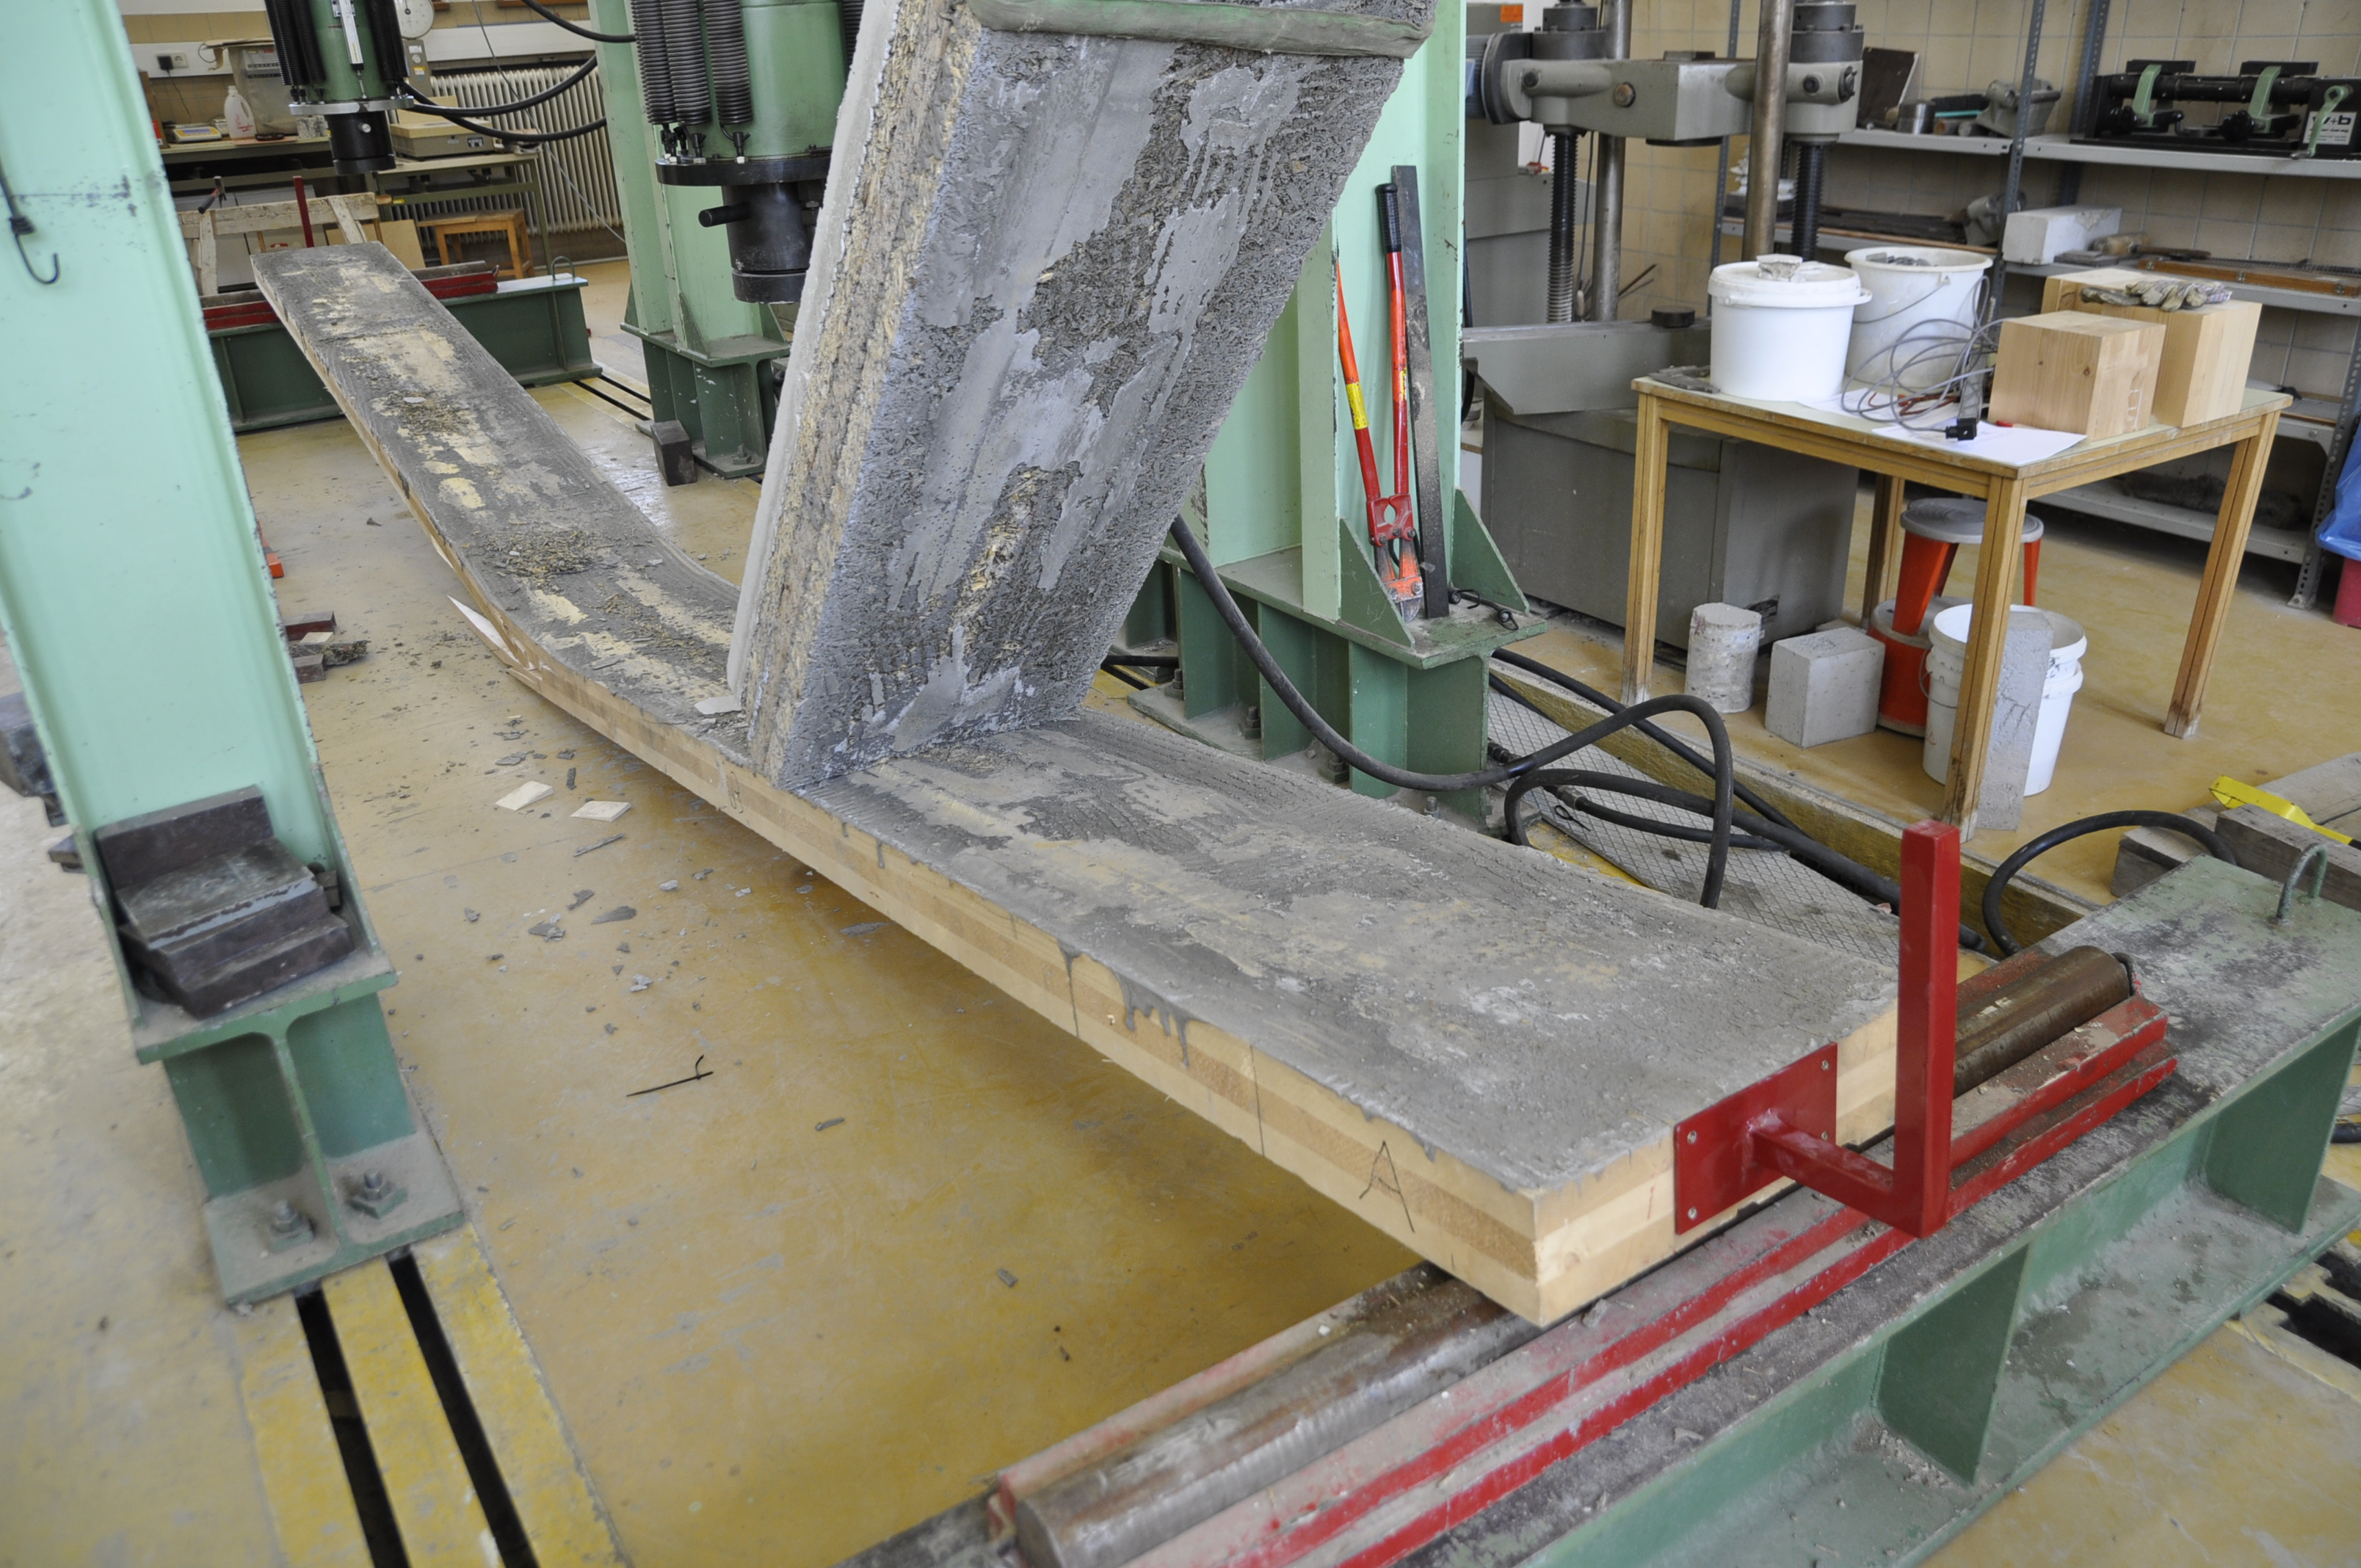
\includegraphics[scale=0.05]{a/A.JPG}
\caption{lustige Dinge}
\label{ka}
\end{center}
\end{figure}

\end{document}
